\chapter{Caching Model}
\label{chapter:caching_model}

In order to get a common understanding of caching and the terminology related to the topic, we will go through the basics of caching by describing the architecture of a web system using a cache, present a model based on a timeline that introduces the different events involved in caching and last we list criteria for evaluating a caching technique in order to choose an appropriate technique for a given use case.

\section{Caching Basics}
\label{sec:caching_basics}

In general caching is about storing the result of a computation at a where you are able to retrieve it fast, such that it is possible to get the result fast instead of recomputing it. This basic algorithm is illustrated on figure~\ref{fig:basic-caching} and can be described as following:

\begin{figure*}[ht!]
  \centering
  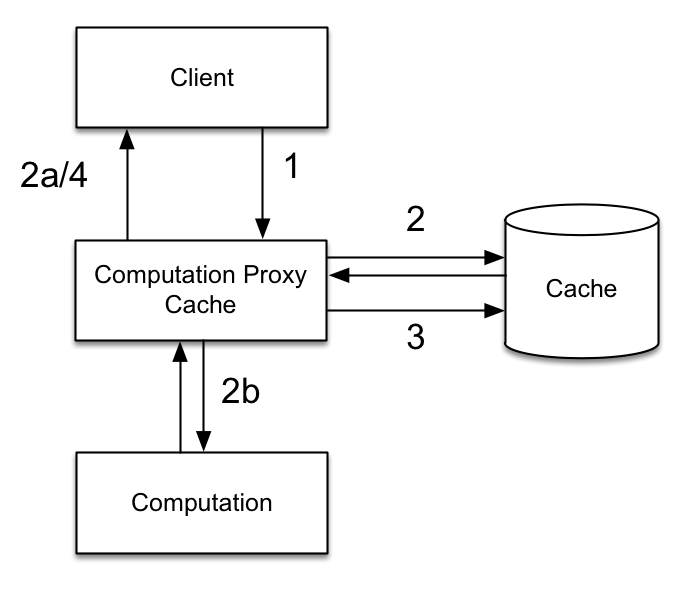
\includegraphics[width=0.6\linewidth]{figures/basic-caching-figure.pdf}
  \begin{enumerate}
    \item The result $v$ of a computation $f$ is requested.
    \item If $v$ is cached and is valid, we go to 5 with $v'=v$. Else we continue.
    \item We run the computation $f$
    \item The new result $v'$ of $f$ is stored in the cache.
    \item $v'$ is returned.
  \end{enumerate}
  \caption{The flow of basic caching}
  \label{fig:basic-caching}
\end{figure*}

In some cases, where the client is not allowed to wait for the computation to run, step 3-4 are replaced by a step that simply returns an empty value.

If we look at the cached value from an abstract point of view, we can see it as a \emph{result of a function} given certain \emph{inputs}. Sometimes the inputs are data from a storage system, sometimes it's the result of an API call to some external resource, sometimes it's global variables in the code. These \emph{inputs} we from now on be referred to as \emph{underlying data}.

In order for the algorithm to work, we need to be sure that when we store the cached value it has to be uniquely identified by some key such that when we lookup the value as in step 2 of the algorithm, we always locate $v$. This presents one of the challenges of cache management, which is in many cases closely related to cache invalidation (one of the two hard things in computer science\footnote{Not scientifically, but at least a favorite saying of Martin Fowler and quote by Phil Karlton}).

In the algorithm cache invalidation is simply described as a \emph{check}, but in reality this is the hard challenge of caching. The \emph{check} could be a precomputed indicator from earlier triggers, it could be based on a key derived from the underlying data or some timestamp. These cache invalidation approaches will be described more in section~\ref{sec:invalidation_techniques}.

\subsection{Architecture}
\label{subsec:architecture}

\begin{figure*}[ht!]
  \centering
  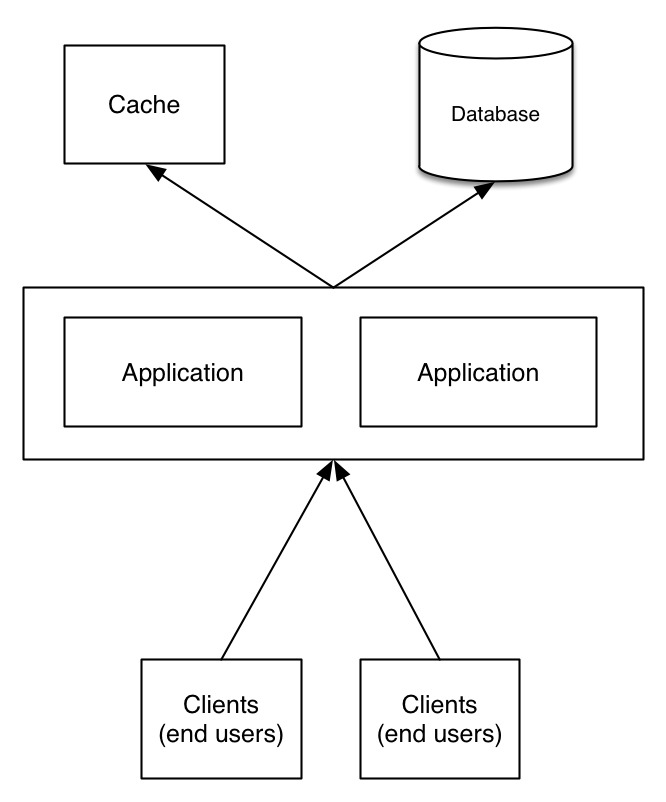
\includegraphics[width=0.5\linewidth]{figures/architecture.pdf}
  \caption{The assumed architecture of the system}
  \label{fig:caching-basics-architecture}
\end{figure*}

The architecture of the web application in which the cache is used is important to how the cache system. We assume that the architecture of the system is a common web application architecture as illustrated in figure~\ref{fig:caching-basics-architecture} consisting of a web application that serves HTTP-requests from the client (represented by the user) and interacts with a primary storage database to store and load data. To store and fetch the cached content we introduce a cache database. This could easily be the same unit as the primary storage database, but we separate them for better clarification.

Most modern web applications needs to serve multiple users at the same time, which means the web application must run on multiple processes\footnote{This is processes as an abstract term used in distributed systems. If we need to be implementation specific this could just as well be threads.} either on a single or multiple machines. We will therefore treat the web application as a distributed system.

A popular choice for cache databases are key-value stores such as Redis~\footnote{http://redis.io/} and Memcached~\footnote{https://memcached.org/} since they are simple distributed key-value stores that lives in memory and therefore allows for scalability and high-performance operations. In order to support most practical web applications, we will therefore make the assumption that the cache database has the same functionality: it should be possible to store arbitrary content for a given key. Furthermore the final solution of this thesis require the cache database to support atomic transactions for a given key, which are supported in Memcached using the CAS command~\cite{docs:memcached-protocol} and in Redis using the \verb$WATCH$-command~\cite{docs:redis-transactions}. The reasons behind this assumption will be explained more in chapter~\ref{chapter:update_propagation}.

% subsection architecture end

\subsection{Timeline Model}
\label{subsec:timeline_model}

As with the algorithm on figure~\ref{fig:basic-caching}, caching can be described by a series of events. The ordering of events decides whether the cached content or a fresh computation is presented to the client. To describe the different caching techniques, we will use a timeline model with a stream of events. One timeline describes the events occurring in a single process. We can therefore assume that there exists a total ordering of events for a single timeline. To be able to describe the caching techniques explained in this thesis, we will define the following events:

\begin{itemize}
  \item \textbf{Requested} is the event occurring when a client requests a given cached value
  \item \textbf{Computation Started} is when the computations is started
  \item \textbf{Computation Finished} is when the computation is finished and a result is returned
  \item \textbf{Stored} is happening when a given is stored in the cache database on a given key
  \item \textbf{UD Updated} is when the underlying data has been updated
  \item \textbf{Invalidated} is when the system has invalidated a cached value
\end{itemize}

To show how the timeline model works, we will give an example involving the different events:

\begin{example}
\label{example:timeline-model}
We will give an example using the basic caching algorithm described on figure~\ref{fig:basic-caching}. Consider the case illustrated on figure~\ref{fig:timeline-example}, where a client requests a value $v$ that at first isn't cached. This means the system will execute the function $f$, which returns the value instance $v_1$ and stores it in the caching database. After this some underlying data involving the computation of $v$ is updated and after the update, the client makes another request for $v$. At this point $v_1$ is not fresh since the execution of $f$ would result in another value. Therefore $v$ is invalidated by the system after which we recompute $f$ and stores the resulting value $v_2$ in the cache database.

\begin{figure*}{ht!]
  \centering
  \includegraphics{width=1.0\linewidth]{figures/timeline-example.pdf}
  \caption{Example of the timeline model}
  \label{fig:timeline-example}
\end{figure*}

\end{example}

% Introduce the timeline and relevant events:
%   - Value registration
%   - Invalidation
%   - Cache update
%   - Value request
% Concurrent Timelines:
%   - Show that we when we have the given architecture, we have
%     multiple concurrent timelines running as in a distributed system
%     => We can assume that each timeline is a process

% subsection timeline_model end

% section caching_basics end

\section{Evaluating Caching Techniques}
\label{sec:evaluating_caching_techniques}

% Goals
% - What are the goals of caching:
% - We don't want the users to wait (/ performance)
% - Use less CPU

% From that desirable properties:
% - Freshness
%   - fresh is better, stale is worse
% - Consistency
%   - cached content should be as consistent with the rest of the system as possible
% - Ease of management (for the developer)
%   - The less effort (= code + thinking/complexity) to cache a given result, the better
%   - We don't want errors, when the related code is changed/extended
%     => E.g. if a new developer introduces a new data source, it should not break
%     => Or at least it should be as easy to detect these things as possible
% - Cache hit rate
%   - This depends on the amount of updates to the underlying data
%   - We can separate between:
%     - The user (have to / does not have to) wait for a given computation every time it is updated
%       => Have to: bad for cached content that is frequently updated + long running computations
%       => Not have to: great for long computations
%     -

% List how we evaluate the different caching techniques to find the right
% technique for the given use case

% - Evaluating caching technique
%   - Freshness
%   - Consistency
%   - Ease of management (invalidation)
%   - Have to wait for computation?

% section evaluating_caching_techniques end

% chapter caching_model end

